\documentclass[border=5mm]{standalone}
\usepackage{pgfplots}

\begin{document}
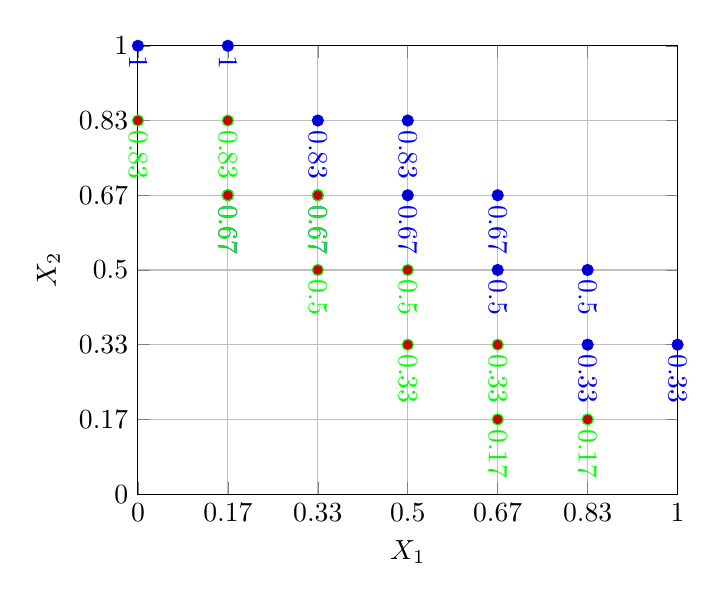
\begin{tikzpicture}
    \begin{axis}[
        xmin=0, xmax=1,
        ymin=0, ymax=1,
        xtick={0,1/6,...,1},
        ytick={0,1/6,...,1},
        grid=major,
        xlabel=$X_1$,
        ylabel=$X_2$,
        nodes near coords,
        every node near coord/.append style={anchor=west, rotate=-90}
    ]
        % Blue ladder
        \addplot+[
            only marks,
            mark=*,
            point meta=y,
            color=blue
        ] coordinates {
            (0,1)   (1/6,1)
            (1/6,4/6) (2/6,4/6)
            (2/6,5/6) (3/6,5/6)
            (3/6,4/6) (4/6,4/6)
            (4/6,3/6) (5/6,3/6)
            (5/6,2/6) (6/6,2/6)
        };

        % Green ladder
        \addplot+[
            only marks,
            mark=*,
            point meta=y,
            color=green
        ] coordinates {
            (0,5/6) (1/6,5/6)
            (1/6,4/6) (2/6,4/6)
            (2/6,3/6) (3/6,3/6)
            (3/6,2/6) (4/6,2/6)
            (4/6,1/6) (5/6,1/6)
        };
    \end{axis}
\end{tikzpicture}
\end{document}